\chapter{Beyond the Standard Model}
\label{chap:BSM}

Although the \ac{SM} represents our best understanding of the elementary particles and their interactions, it does contain some deficiencies. On the one hand, it remains silent on some important phenomena, such as gravity, dark matter, and dark energy. On the other hand, several anomalies have emerged from recent experiments, those in the flavor sector in particular. Two of the experimental results in the flavor sector that work against the \ac{SM} and their phenomenological implications are discussed in \autoref{sec:BSM}. \autoref{sec:Leptoquark} introduces the leptoquark model that can be used to explain the unexpected results that occurred in the flavor sector.

\section{BSM Phenomenology}
\label{sec:BSM}

As discussed in \autoref{sec:Flavor}, the renormalizable \ac{SM} Lagrangian exhibits a few continuous global symmetries, namely the $U(1)_{e}\bigotimes U(1)_{\mu}\bigotimes U(1)_{\tau}$ that gives rise to the conservation of lepton family numbers. Unlike gauge symmetries of the \ac{SM}, which arise at the outset of the construction, these global $U(1)$ symmetries emerge accidentally due to the assumption (massless neutrino) that is solely driven by phenomenology. Despite the accidental nature of these symmetries, they have stood up to the tests of almost all particle physics experiments to date.  

In fact, the first and so far the only hint of the broken global symmetries did not appear until the turn of the century through the oscillation of atmospheric neutrinos \cite{Super-Kamiokande:1998kpq,SNO:2002tuh}. Figure~\ref{fig:SuperK} shows the strong evidence of neutrino oscillations presented by the Super-Kamiokande Collaboration. This remarkable observation directed significant interest from both theorists and experimentalists to the flavor sector of the \ac{SM}. On the one hand, it cements the calls for extensions of the \ac{SM} by demonstrating the mixing of neutrino flavors. On the other hand, it also suggests that the $U(1)$ symmetries are indeed broken, and the \ac{CLFV} is also expected to occur. 

\begin{figure}[tbh!]
 \begin{center}
 \begin{tabular}{c}
 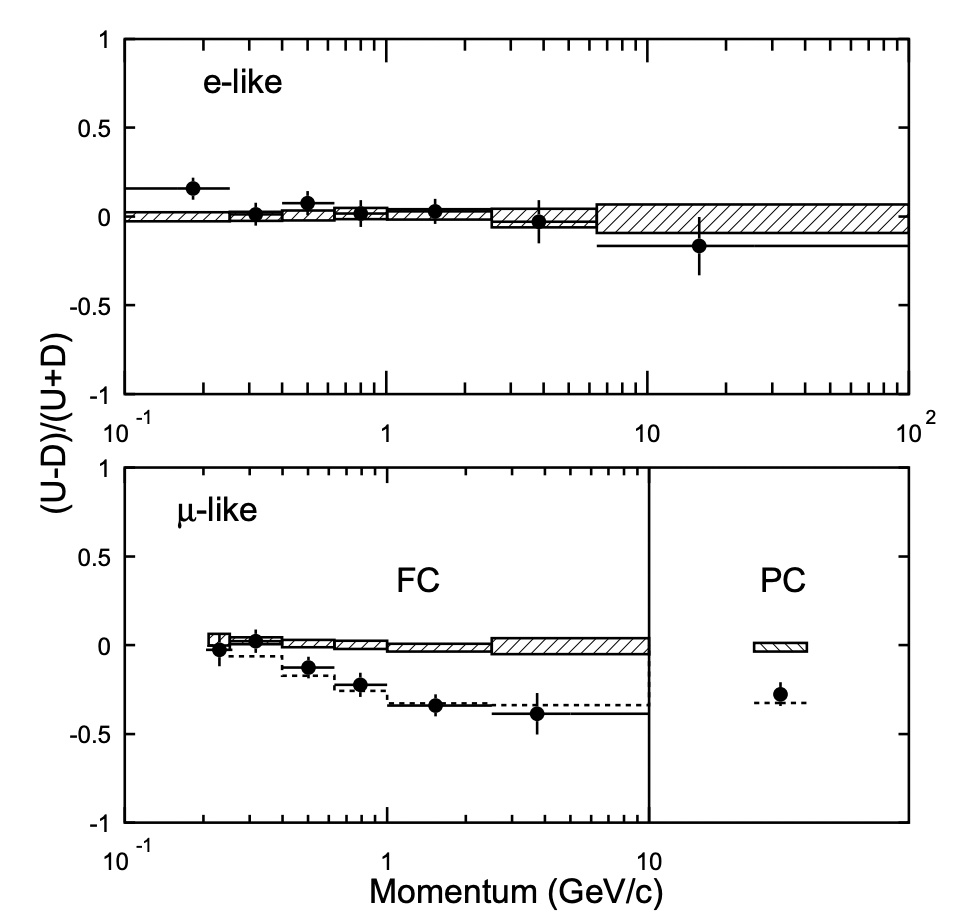
\includegraphics[width=0.6\textwidth]{figures/Part1/BSM/SuperK}
 \end{tabular}
 \caption{Evidence of neutrino oscillation presented by the Super-Kamiokande Collaboration in 1998~\cite{Super-Kamiokande:1998kpq}. The asymmetry in the zenith angle is plotted as a function of momentum for $e$-like events (upper panel) and $\mu$-like events. The data are represented with filled points. The expected distributions under the hypothesis of no neutrino oscillation are shown with filled bands while the dashed line is the expected distribution for the alternative hypothesis.}
 \label{fig:SuperK}
 \end{center}
\end{figure}

Although the exact mechanism behind neutrino mass remains unclear, it can be induced through two distinct ways that only require minimal departures from the original formulation of the \ac{SM}. By adding right-handed neutrino fields, the Yukawa coupling \cite{Weinberg:1967tq} that describes the emergence of Dirac fermion masses can be naturally extended to neutrinos. The neutrino mass can also be realized by introducing an effective operator~\cite{Weinberg:1979sa}, sometimes referred to as the Weinberg operator. This operator gives rise to Majorana neutrino mass terms upon spontaneous symmetry breaking. This operator is however nonrenormalizable, meaning its underlying theory is valid only up to a specific energy scale. Nevertheless, it can be viewed as an effective description of high-energy physics at a low-energy scale. This type of approach is known as the \ac{EFT}, which is discussed further in \autoref{chap:EFT}.

In either case, the mass of neutrinos is accounted for and Equation~\ref{eq:Yukawa} can be subsequently updated to include neutrino mass terms. The presence of massive neutrino fields also means that the \ac{PMNS} matrix introduced in \autoref{sec:Flavor} will no longer be fully diagonal, for the same reason why the \ac{CKM} matrix contains off-diagonal elements. The strength of the neutrino flavor mixing is therefore governed by the off-diagonal elements of the \ac{PMNS} matrix -- a nearly perfect analog to the \ac{CKM} matrix. 

The same \ac{PMNS} matrix can also give rise to the \ac{CLFV} process through loop diagrams involving charged current, as illustrated in Figure~\ref{fig:mutoe}. However, these diagrams are highly suppressed and phenomenologically negligible due to the small neutrino mass relative to the \ac{EW} scale. Therefore, any experimental observation of \ac{CLFV} will be unambiguous evidence of new physics beyond the \ac{SM}.

\begin{figure}[tbh!]
 \begin{center}
 \begin{tabular}{c}
 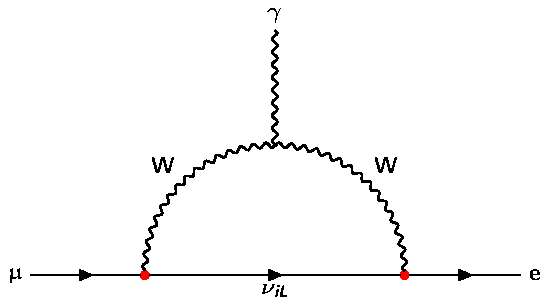
\includegraphics[width=0.7\textwidth]{figures/Part1/BSM/mutoe}
 \end{tabular}
 \caption{Feynman diagram that shows $\upmu\rightarrow$e transition via W loop. The \ac{PMNS} matrix elements enter this diagram through the starting and end points in the W loop, indicated with red dots. The index $i$ runs over lepton generations.}
 \label{fig:mutoe}
 \end{center}
\end{figure}

Recent tests of lepton flavor universality conducted by the \ac{LHCb}~\cite{LHCb:2023zxo} and various other experiments~\cite{HFLAV} in the b$\rightarrow$c transitions established a mild tension (3$\sigma$) with respect to the \ac{SM} predictions. These experiments measured the following ratio of branching fractions:

\begin{equation}
\mathcal{R}(\textsf{D})=\frac{\mathrm{\Gamma}(\textsf{B}\rightarrow\textsf{D}\uptau^{-}\bar{\nu}_{\uptau})}{\mathrm{\Gamma}(\textsf{B}\rightarrow\textsf{D}\upmu^{-}\bar{\nu}_{\upmu})},
\end{equation}

which is sensitive to new physics where the flavor structure is different.

\begin{figure}[tbh!]
 \begin{center}
 \begin{tabular}{c}
 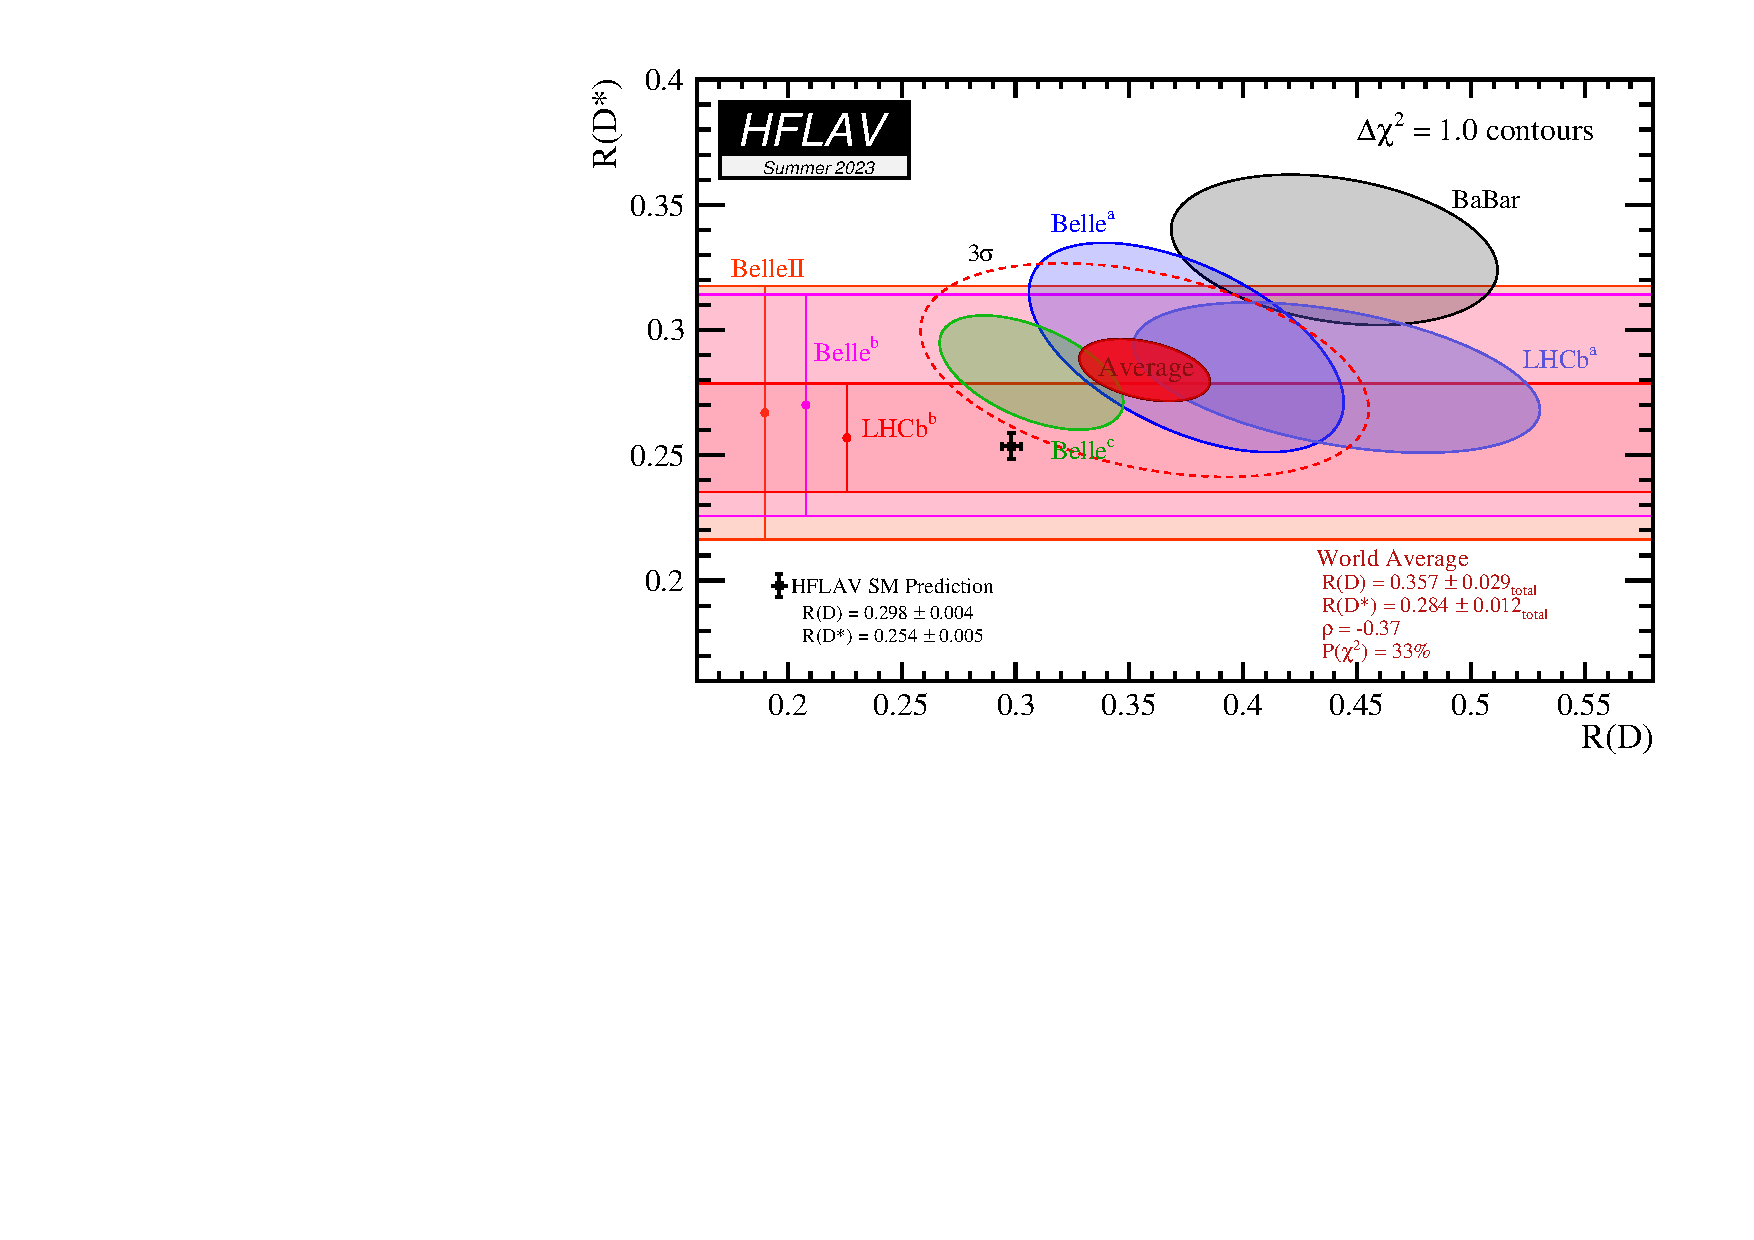
\includegraphics[width=0.7\textwidth]{figures/Part1/BSM/RD}
 \end{tabular}
 \caption{Recent results on $\mathcal{R}(\textsf{D})$ and $\mathcal{R}(\textsf{D}^{*})$ measurements compiled by the HFLAV Group~\cite{HFLAV}. Results are shown in a two-dimensional plane with the x-axis and y-axis representing $\mathcal{R}(\textsf{D})$ and $\mathcal{R}(\textsf{D}^{*})$, respectively. Contours with solid line boundaries represent results published by various experiments. The world average is shown in the middle. The 3$\sigma$ contour is represented with a red dashed line. The \ac{SM} prediction is represented with a data point with error bars.}
 \label{fig:RD}
 \end{center}
\end{figure}

This anomaly is known as the ``$\mathcal{R}(\textsf{D})$'' anomaly and its situation as of Summer 2023 is summarized in Figure~\ref{fig:RD}. As discussed in \autoref{sec:Flavor}, the coupling strength of the weak charged current does not distinguish between lepton flavors. However, results from these measurements seem to suggest the W$\rightarrow\uptau\nu$ decay channel is favored over W$\rightarrow\upmu\nu$ decay channel. Not only did these measurements provide a direct hint towards \ac{LFUV}, it also prompted renewed experimental interest in \ac{CLFV} search since models that accommodate \ac{LFUV} generally give rise to \ac{CLFV} as well~\cite{Glashow:2014iga}. 

\section{Leptoquark Model}
\label{sec:Leptoquark}

Leptoquarks are hypothetical scalar or vector bosons that were first proposed nearly half a century ago~\cite{Pati:1973uk}. They are simultaneously charged with color, isospin, and hypercharge quantum numbers, and thus can mediate lepton-quark couplings. When imposing the \ac{SM} \sm~gauge symmetry, a large pool of possible leptoquark candidates can be reduced to six scalar leptoquarks and six vector leptoquarks~\cite{Dorsner:2016wpm}, which is summarized in Table~\ref{tab:Leptoquark}. 

\begin{table}[th]
\sffamily
\centering
\caption{Possible leptoquark candidates that respect \sm~gauge symmetry, summarized in~\cite{Dorsner:2016wpm}. The spin-0 fields correspond to scalar leptoquark while spin-1 fields correspond to vector leptoquark.}
\begin{tabular}{cccc}
\toprule 
$(SU(3), SU(2), U(1))$ & Spin  & Symbol & Type \\ \midrule
($\bar{\bm{3}}$, $\bm{1}$, -2/3) & 0 & $\bar{S}_{1}$ & $\overline{RR}(\bar{S}_{0}^{\bar{R}})$ \\
($\bar{\bm{3}}$, $\bm{1}$, 1/3) & 0 & $S_{1}$ & $LL(S_{0}^{L})$, $RR(S_{0}^{R})$, $\overline{RR}(S_{0}^{\bar{R}})$ \\
($\bar{\bm{3}}$, $\bm{1}$, 4/3) & 0 & $\tilde{S}_{1}$ & $RR(\tilde{S}_{0}^{R})$ \\
($\bm{\bm{3}}$, $\bm{2}$, 1/6) & 0 & $\tilde{R}_{2}$ & $RL(\tilde{S}_{1/2}^{L})$, $\overline{LR}(\tilde{S}_{1/2}^{\bar{R}})$ \\
($\bar{\bm{3}}$, $\bm{2}$, 7/6) & 0 & $R_{2}$ & $RL(S_{1/2}^{L})$, $LR(S_{1/2}^{R})$ \\
($\bar{\bm{3}}$, $\bm{1}$, -2/3) & 0 & $S_{3}$ & $LL(S_{1}^{L})$\\
\midrule
($\bm{3}$, $\bm{1}$, -1/3) & 1 & $\bar{U}_{1}$ & $\overline{RR}(\bar{V}_{0}^{\bar{R}})$ \\
($\bm{3}$, $\bm{1}$, 2/3) & 1 & $U_{1}$ & $LL(V_{0}^{L})$, $RR(V_{0}^{R})$, $\overline{RR}(V_{0}^{\bar{R}})$ \\
($\bm{3}$, $\bm{1}$, 5/3) & 1 & $\tilde{V}_{1}$ & $RR(\tilde{V}_{0}^{R})$ \\
($\bar{\bm{3}}$, $\bm{2}$, -1/6) & 1 & $\tilde{V}_{2}$ & $RL(\tilde{V}_{1/2}^{L})$, $\overline{LR}(\tilde{V}_{1/2}^{\bar{R}})$ \\
($\bar{\bm{3}}$, $\bm{2}$, 5/6) & 1 & $V_{2}$ & $RL(V_{1/2}^{L})$, $LR(V_{1/2}^{R})$ \\
($\bm{3}$, $\bm{3}$, 1/3) & 1 & $U_{3}$ & $LL(V_{1}^{L})$\\
\bottomrule
\end{tabular}
\vspace{-0.5em}
\label{tab:Leptoquark}
\end{table}

A lot of phenomenological interests have gravitated towards the leptoquark models recently due to the emergence of $\mathcal{R}(\textsf{D})$ anomaly. Taking the $U_{1}$ leptoquarks as an example. Assuming they only interact with left-handed fermions, the interaction term can be written as:

\begin{equation}
\lambda\beta^{ij}_{L}\bar{Q}_{L}^{i}\gamma^{\mu}L_{L}^{j}U_{1\mu},
\end{equation}

where $\lambda$ is the coupling strength, and $\beta^{ij}_{L}$ is a 3$\times$3 matrix that encodes the flavor structure of $U_{1}$ interactions. This term can contribute at the tree level to the b$\rightarrow$c transitions where the anomaly is reported. A side-by-side comparison of Feynman diagrams for the \ac{SM} and leptoquark contributions to this process is shown in Figure~\ref{fig:Leptoquark}.

\begin{figure}[tbh!]
 \begin{center}
 \begin{tabular}{cc}
 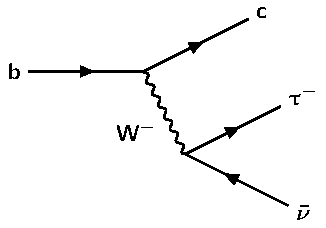
\includegraphics[width=0.45\textwidth]{figures/Part1/BSM/SMbtoc}&
 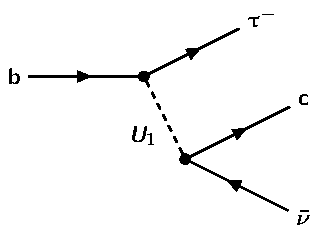
\includegraphics[width=0.45\textwidth]{figures/Part1/BSM/U1}\\
 \end{tabular}
 \caption{Representative Feynman diagram for tree-level $\textsf{b}\rightarrow\textsf{c}\uptau\nu$ transition. The \ac{SM} contribution is shown on the left. Possible contributions from the $U_{1}$ leptoquark, represented with a dashed line in the diagram, are shown on the right.}
 \label{fig:Leptoquark}
 \end{center}
\end{figure}

An explanation of the $\mathcal{R}(\textsf{D})$ anomaly is possible if $U_{1}$ leptoquarks interact strongly with the third generations while leaving out or interacting very weakly with the first and second generations. In other words, a $\beta^{ij}_{L}$ matrix of the form

\begin{equation}
\begin{pmatrix}
0 & 0 & 0\\
0 & \mathcal{O}(0.01) & \mathcal{O}(0.1)\\
0 & -\mathcal{O}(0.1) & 1\\
\end{pmatrix},
\end{equation}

could be used to explain the $\mathcal{R}(\textsf{D})$ anomaly, as pointed out by Ref.~\cite{Cornella:2021sby}. Direct searches for leptoquarks decaying into tau leptons (i.e. third generation) have been performed by both \ac{ATLAS}~\cite{ATLAS:2023uox,ATLAS:2023vxj} and \ac{CMS}~\cite{CMS:2018txo,CMS:2023qdw} Collaborations, and so far no conclusive evidence has been reported.

Secondly, the leptoquark model provides an interesting connection between the $\mathcal{R}(\textsf{D})$ anomaly and flavor-changing phenomena at a higher energy scale. For example, the $\mathcal{R}(\textsf{D})$ anomaly can also be explained by the $S_1$ leptoquark listed in Table~\ref{tab:Leptoquark}. Because $S_1$ can interact with left-handed fields, the b quark and neutrino in the interaction vertex can be replaced with a top quark and a muon, as illustrated in Figure~\ref{fig:S1}. This results in the flavor-violating t$\rightarrow\ell\ell^{\prime}$q decay, which is strongly suppressed in the \ac{SM} by the mass hierarchy of both quarks and leptons. It was suggested in Ref.~\cite{Kim:2018oih} that the $\mathcal{R}(\textsf{D})$ anomaly, if true, can give rise to a sizable rate of \ac{CLFV} events, which reaches $\mathcal{O}(10^{-6})$ at tree-level for t$\rightarrow\ell\ell^{\prime}$c process involving a top quark.

\begin{figure}[tbh!]
 \begin{center}
 \begin{tabular}{cc}
 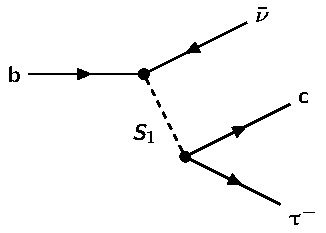
\includegraphics[width=0.45\textwidth]{figures/Part1/BSM/S1}&
 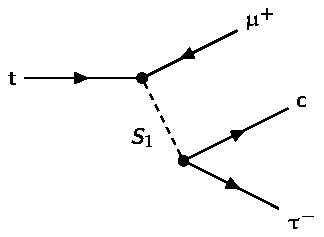
\includegraphics[width=0.45\textwidth]{figures/Part1/BSM/S1x}\\
 \end{tabular}
 \caption{Feynman diagrams of processes mediated by $S_1$ leptoquark, represented with a dashed line in both diagrams. The left diagram shows a possible explanation for $\mathcal{R}(\textsf{D})$ anomaly offered by the $S_1$. The same $S_1$ can give rise to \ac{CLFV} in the top quark sector, which is shown on the right.}
 \label{fig:S1}
 \end{center}
\end{figure}

Finally, the \ac{CERN} \ac{LHC} can provide sensitivity to \ac{CLFV} searches in two- or three-body decays of heavy particles, X$\rightarrow\ell\ell^{\prime}$(Y), and in heavy-particle production, pp$\rightarrow\ell\ell^{\prime}$X. Here, X refers to a heavy \ac{SM} particle such as a top quark or a Higgs, W, or Z boson, Y denotes an additional generic \ac{SM} particle. For \ac{CLFV} processes involving the heaviest of all elementary particles, the top quark, competitive sensitivity is predicted at the \ac{LHC} compared to previous bounds on such interactions~\cite{Davidson:2015zza}. Therefore, a search for \ac{CLFV} in the top quark sector at the \ac{LHC} could shed light on these flavor anomalies and further our understanding of the broken global symmetries.